\part{More technical details}
\label{part:technical_details}


%------------------------------------
\section{Data to be used}
\label{sec:data}

In an ideal scenario, the GAN would make use of custom training data collected for this assignment.
Some technical detail about the required training data, which are images, is given below:
\begin{itemize}
    \item Should be of JPG format.
    \item Should have a maximum resolution of 512x512, preferably even lower (limited computational power).
    \item Should be of cars from a European brand, Peugeot and Mercedes in particular.
    \item Should contain the same car in diverse angles.
    \item Would ideally be labelled with brand, model, colour, body type and release year. The more meta-data the merrier.
    \item From the literature study it seems over 50 thousand images per brand should be needed, \textit{as a minimum}.
\end{itemize}

The images could be scraped from the web.
Thus a custom scraper would need to be written to collect images.
The scraper should work by using popular car auction websites since these would allow for collecting meta-data as well.

While collecting training data for the project would be ideal, this would require a considerable amount of time.
Luckily, if it would turn out unfeasible to do this, many existing pre-bundled training sets exist.
The LSUN-Stanford Car Dataset by \citet{cardb} could be used, as discussed in the previous assignment.
This dataset consists of over 2 million images.

The only drawback of using the LSUN-Stanford Car Dataset is that it consists of images from multiple, mostly American, car brands.
My personal knowledge of these is lesser than my knowledge of European car brands.
This could impose some issues for the evaluation portion of this project since it would be harder to assess if the generated image resembles an existing car.
However, this can be minimized by having enough juries with expertise to evaluate the images.
This will be discussed in greater detail in the next assignment. 

In both of these cases, the used training data would have been already publicly available so there are no expected issues for licensing.


%------------------------------------
\clearpage
\section{Required components and flow of the system}
\label{sec:required_components}

As was already discussed in the previous assignments, the following components are required and will be used from top to bottom:

\begin{itemize}
    \item A crawler that collects input training images from the web.
    \begin{itemize}
        \item Can be bypassed by using LSUN-Stanford Car Dataset.
    \end{itemize}
    \item A DCGAN that generates images of cars based on the collected training images.
    \begin{itemize}
        \item The official TensorFlow implementation of StyleGan2 will be used for this \citep{stylegan2}.
        \item The computational requirement for this is rather gigantic. Luckily a pre-trained car GAN exists as already discussed in the previous assignment. Those could be used as-is or they can be further fine-tuned.
    \end{itemize}
    \item A framework that allows for control over the GAN.
    \begin{itemize}
        \item Since the resulting GAN is of the black-box principle, control over the AI is hard, however, not impossible.
        \item Some research was already done in the previous assignment surrounding control over hidden layers. Since then, a paper that talks about the development of a GUI for this purpose has caught my attention, GANSpace \citep{ganspace}.
        \item GANSpace is compatible with StyleGan2 \citep{ganspace} and supplies an easy-to-use interface.
        \item GANSpace has a demo over the pre-trained StyleGan2 car-related GAN, shown in figure \ref{fig:ganspace}.
    \end{itemize}
    \item An online questionnaire.
    \begin{itemize}
        \item Allows getting human feedback on whether or not the resulting cars look like actual cars.
        \item A tool previously created by me can be modified to hold this survey in a randomised fashion \citep{bapproef}.
        \item More details about this tool will be given in the next assignment.
    \end{itemize}
\end{itemize}

\begin{figure*}
\centering
\begin{subfigure}{.45\textwidth}
  \centering
  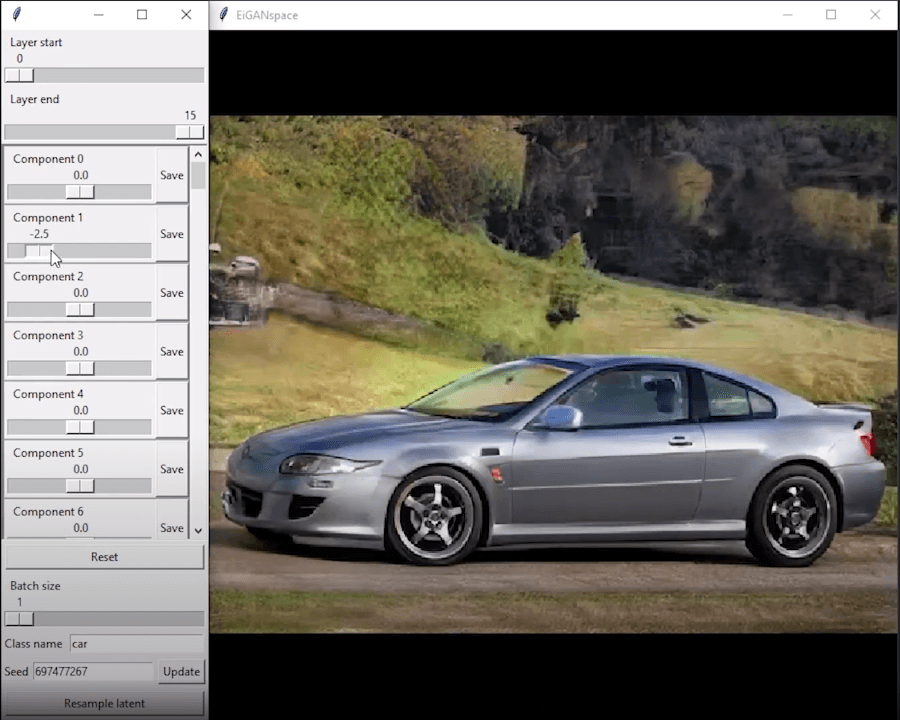
\includegraphics[width=\textwidth]{images/ganspace_1.png}
  \caption{Two door coupe}
  \label{fig:twodoor}
\end{subfigure}%
\hspace{1cm}
\begin{subfigure}{.45\textwidth}
  \centering
  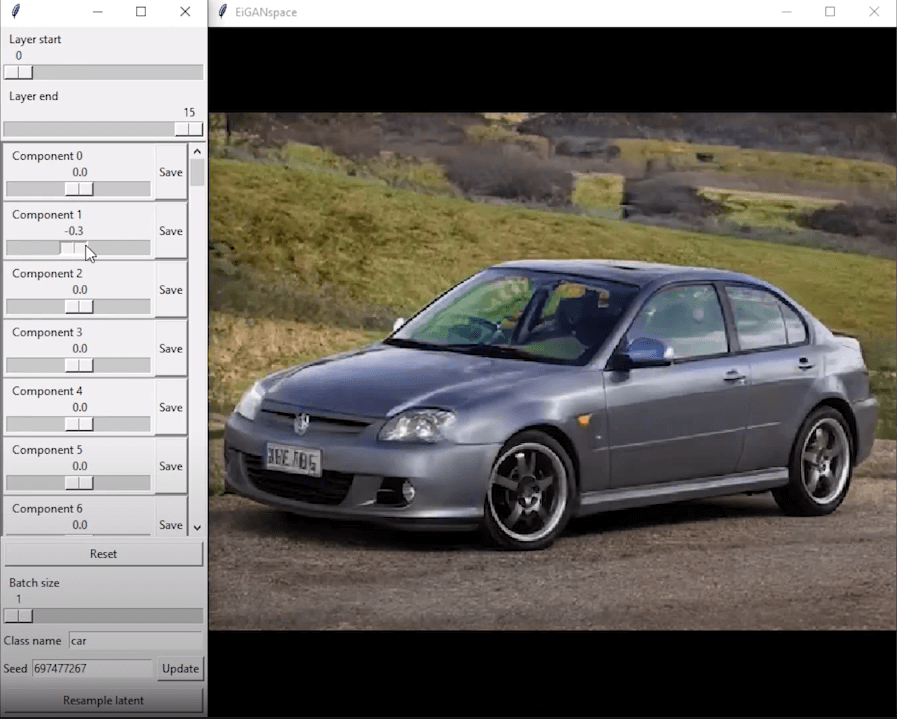
\includegraphics[width=\textwidth]{images/ganspace_2.png}
  \caption{Four door sedan}
  \label{fig:fourdoor}
\end{subfigure}
\captionsetup{width=.85\linewidth}
\caption{Fragments of the GANSpace demo demonstrating the control over the AI to generate similar looking cars with different properties \citep{ganspacevid}.}
\label{fig:ganspace}
\end{figure*}